\documentclass[10pt,letterpaper]{article}
\usepackage{amssymb}
\usepackage{amsmath}
\usepackage{graphicx}
\usepackage{booktabs}
\usepackage{float}
\title{HW1}
\author{ZONGQI CUI}
\begin{document}
\maketitle
\begin{itemize}
    \item {1.}
        \begin{itemize}
            \item {ordinary least squares regression}
                \[\beta^{ols} = \arg\min\sum_{i=1}^{n}  \]
                we transform it to matrix:
                \[\beta^{ols} = \arg\min(y-X \beta )^T(y-X \beta ) \]
                we can get :
                \[\beta^{ols} =(X^TX)X^Ty\]
                $\because$ The augmented dataset is created by extending the centered matrix \textbf{X} with k additional rows, with the value  $\sqrt{\lambda }I$, and by augmenting the vector
                y with k zeros.\\
                $\therefore $ we can get:
                    \[\tilde{X} =\binom{X}{\sqrt{\lambda }I} \]
                    \[\tilde{y} =\binom{y}{0} \]\\
                $\because$From above we can get:\[\beta^{ols} =(X^TX)X^Ty\]\\
                $\therefore$
                \[\beta^{ols} =(\tilde{X}^T\tilde{X})\tilde{X}^T\tilde{y}\]\\
                $\because$
                \[\tilde{X}^T \tilde{X} = \begin{bmatrix} X^T & \sqrt{\lambda}I^T \end{bmatrix}\begin{bmatrix} X \ \sqrt{\lambda}I \end{bmatrix} = X^TX + \lambda I \]
                \[\tilde{X}^T\tilde{y}=\begin{bmatrix}
                    X^T & \sqrt{\lambda}I^T
                \end{bmatrix}
                \begin{bmatrix}
                    y \\
                    0
                \end{bmatrix}=
                X^Ty\]\\
                $\therefore$
                \[\beta^{ols}=(X^TX+\lambda I)^-1XT^y\]
            \item {Ridge regression}
                $\because$
                \[\beta^{ridge}=(X^TX+\lambda I)^-1XT^y\]
                $\therefore$
                adding these rows the ordinary regression will end up with the same coefficients as (regularized) ridge regression.
        \end{itemize}
    \newpage
    \item {2(a)}
        \begin{itemize}
            \item {1.load data}\\
            load data into file
            \item {2.standardized data}\\
            make everydata in int64 type and standardized them
        \end{itemize}
    \newpage
    \item {2(e)}
    In this section, we report the Root Mean Squared Error (RMSE) and \(R^2\) scores for Model 2c and Model 2d on the training, validation, and test sets. The results are summarized in Table~\ref{tab:rmse_r2_comparison}.

                \begin{table}[H]
                \centering
                \begin{tabular}{lcccc}
                \toprule
                \textbf{Set}     & \textbf{Metric} & \textbf{Model 2c} & \textbf{Model 2d} \\
                \midrule
                \textbf{Train}   & RMSE            & 98.94             & 99.87            \\
                                & \(R^2\)         & 0.17             & 0.16            \\
                \midrule
                \textbf{Validation} & RMSE         & 97.72             & 89.66            \\
                                & \(R^2\)         & -0.001            & 0.16            \\
                \midrule
                \textbf{Test}    & RMSE            & 97.04             & 85.93            \\
                                & \(R^2\)         & -0.14            & 0.11            \\
                \bottomrule
                \end{tabular}
                \caption{Comparison of RMSE and \(R^2\) values between Model 2c and Model 2d.}
                \label{tab:rmse_r2_comparison}
                \end{table}
        \begin{itemize}
            \item The RMSE values suggest that Model 2d performs better across validation and test sets, with lower RMSEs compared to Model 2c.
            \item The \(R^2\) scores also indicate better performance for Model 2d, as its \(R^2\) values are positive across the validation and test sets, whereas Model 2c shows negative \(R^2\) values in both cases.
            \item This suggests that Model 2d generalizes better to unseen data compared to Model 2c, as it explains more variance in the validation and test data, while Model 2c struggles, particularly in the test set.
        \end{itemize}
    \newpage
    \item {2(h)}
    \begin{table}[H]
        \centering
        \begin{tabular}{ccccccc}
        \toprule
        \(\lambda\) & \textbf{Train RMSE} & \textbf{Train \(R^2\)} & \textbf{Val RMSE} & \textbf{Val \(R^2\)} & \textbf{Test RMSE} & \textbf{Test \(R^2\)} \\
        \midrule
        0.0  & 98.94  & 0.17  & 95.87 & 0.04 & 89.21 & 0.04 \\
        0.05 & 98.94  & 0.17  & 95.77 & 0.04 & 89.16 & 0.04 \\
        0.1  & 98.95  & 0.17  & 95.68 & 0.04 & 89.12 & 0.04 \\
        0.15 & 98.97  & 0.17  & 95.59 & 0.04 & 89.06 & 0.04 \\
        0.2  & 98.98  & 0.17  & 95.48 & 0.04 & 88.97 & 0.04 \\
        0.25 & 99.00  & 0.17  & 95.39 & 0.05 & 88.87 & 0.04 \\
        0.3  & 99.02  & 0.17  & 95.30 & 0.05 & 88.76 & 0.05 \\
        0.35 & 99.04  & 0.17  & 95.22 & 0.05 & 88.65 & 0.05 \\
        0.4  & 99.07  & 0.17  & 95.09 & 0.05 & 88.54 & 0.05 \\
        0.45 & 99.10  & 0.17  & 94.97 & 0.05 & 88.43 & 0.05 \\
        0.5  & 99.13  & 0.17  & 94.86 & 0.06 & 88.33 & 0.06 \\
        0.55 & 99.16  & 0.17  & 94.75 & 0.06 & 88.22 & 0.06 \\
        0.6  & 99.20  & 0.17  & 94.67 & 0.06 & 88.12 & 0.06 \\
        0.65 & 99.23  & 0.17  & 94.59 & 0.06 & 88.02 & 0.06 \\
        0.7  & 99.27  & 0.17  & 94.53 & 0.06 & 87.92 & 0.06 \\
        0.75 & 99.31  & 0.17  & 94.47 & 0.06 & 87.83 & 0.07 \\
        0.8  & 99.35  & 0.17  & 94.43 & 0.07 & 87.76 & 0.07 \\
        0.85 & 99.39  & 0.17  & 94.41 & 0.07 & 87.71 & 0.07 \\
        0.9  & 99.43  & 0.17  & 94.39 & 0.07 & 87.66 & 0.07 \\
        0.95 & 99.47  & 0.17  & 94.38 & 0.07 & 87.64 & 0.07 \\
        \bottomrule
        \end{tabular}
        \caption{RMSE and \(R^2\) values for Lasso regression with different \(\lambda\) (alpha) values.}
        \label{tab:lasso_results}
        \end{table}
        
        \begin{table}[H]
        \centering
        \begin{tabular}{ccccccc}
        \toprule
        \(\lambda\) & \textbf{Train RMSE} & \textbf{Train \(R^2\)} & \textbf{Val RMSE} & \textbf{Val \(R^2\)} & \textbf{Test RMSE} & \textbf{Test \(R^2\)} \\
        \midrule
        0.05 & 98.94  & 0.17  & 95.87 & 0.04 & 89.21 & 0.04 \\
        0.1  & 98.94  & 0.17  & 95.87 & 0.04 & 89.21 & 0.04 \\
        0.15 & 98.94  & 0.17  & 95.87 & 0.04 & 89.21 & 0.04 \\
        0.2  & 98.94  & 0.17  & 95.87 & 0.04 & 89.21 & 0.04 \\
        0.25 & 98.94  & 0.17  & 95.87 & 0.04 & 89.21 & 0.04 \\
        0.3  & 98.94  & 0.17  & 95.87 & 0.04 & 89.21 & 0.04 \\
        0.35 & 98.94  & 0.17  & 95.87 & 0.04 & 89.21 & 0.04 \\
        0.4  & 98.94  & 0.17  & 95.87 & 0.04 & 89.21 & 0.04 \\
        0.45 & 98.94  & 0.17  & 95.87 & 0.04 & 89.21 & 0.04 \\
        0.5  & 98.94  & 0.17  & 95.87 & 0.04 & 89.21 & 0.04 \\
        0.55 & 98.94  & 0.17  & 95.87 & 0.04 & 89.21 & 0.04 \\
        0.6  & 98.94  & 0.17  & 95.86 & 0.04 & 89.21 & 0.04 \\
        0.65 & 98.94  & 0.17  & 95.86 & 0.04 & 89.21 & 0.04 \\
        0.7  & 98.94  & 0.17  & 95.86 & 0.04 & 89.21 & 0.04 \\
        0.75 & 98.94  & 0.17  & 95.86 & 0.04 & 89.21 & 0.04 \\
        0.8  & 98.94  & 0.17  & 95.86 & 0.04 & 89.21 & 0.04 \\
        0.85 & 98.94  & 0.17  & 95.86 & 0.04 & 89.21 & 0.04 \\
        0.9  & 98.94  & 0.17  & 95.86 & 0.04 & 89.21 & 0.04 \\
        0.95 & 98.94  & 0.17  & 95.86 & 0.04 & 89.21 & 0.04 \\
        \bottomrule
        \end{tabular}
        \caption{RMSE and \(R^2\) values for Ridge regression with different \(\lambda\) (alpha) values.}
        \label{tab:ridge_results}
        \end{table}
        \begin{itemize}
            \item Conclusion: Lasso shows better performance improvement as 
            $\lambda$ increases, with optimal performance at 
            $\lambda$ = 0.8. Ridge regression, however, shows no significant changes in performance for different 
            $\lambda$ values, suggesting that the regularization effect may not be as impactful for this data in Ridge.
            
        \end{itemize}
    \newpage    
    \item {3(f)}
        \begin{itemize}
            \item {image}
                The plot below shows the objective function value \( f_o(x) \) as a function of the number of epochs for various learning rates \( \eta \), with regularization parameters \( \lambda = 0.8 \) and \( \alpha = 0.5 \).

                \begin{figure}[H]
                    \centering
                    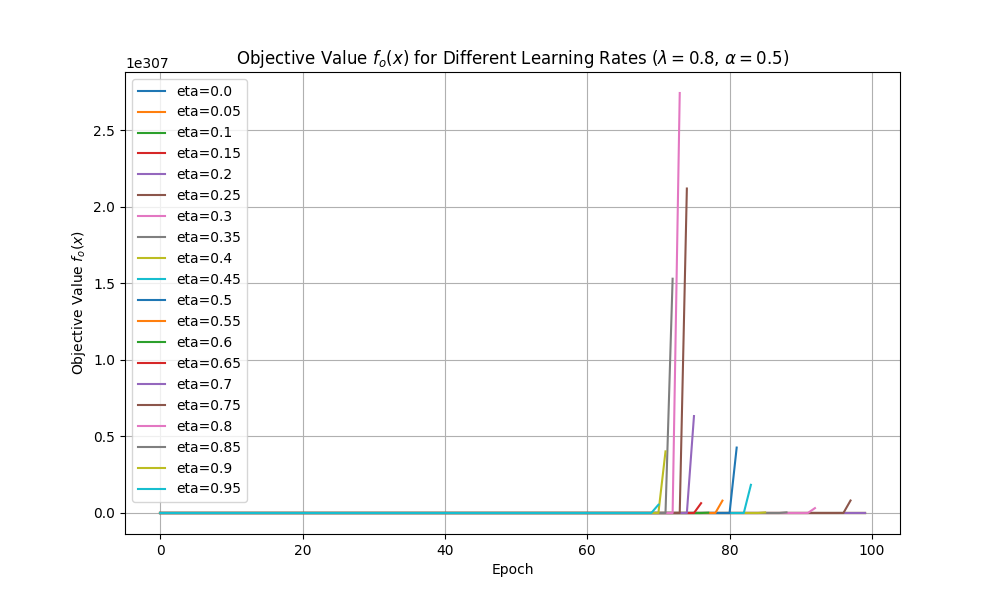
\includegraphics[width=1.4\textwidth]{D:/code/latex/CS534-ml/HW1/Figure_1.png}
                    \caption{Objective Value \( f_o(x) \) for Different Learning Rates (\( \lambda = 0.8, \alpha = 0.5 \))}
                \end{figure}
            
            \item {Conclusion}
            From the plot, smaller learning rates such as \( \eta = 0.05, 0.1, 0.25 \) provide smoother convergence and more stable behavior. \\
            Higher learning rates (\( \eta \geq 0.4 \)) lead to divergence and are unsuitable for this task.
        \end{itemize}
    
    \newpage
    \item {3(g)}
        \begin{table}[H]
            \centering
            \begin{tabular}{ccccccc}
            \toprule
            \textbf{Alpha} & \textbf{Train RMSE} & \textbf{Val RMSE} & \textbf{Test RMSE} & \textbf{Train \(R^2\)} & \textbf{Val \(R^2\)} & \textbf{Test \(R^2\)} \\
            \midrule
            0.00 & 0.4598 & 4.2931 & 2.3111 & 0.9629 & 0.2907 & 0.3828 \\
            0.10 & 0.4598 & 4.2922 & 2.3104 & 0.9629 & 0.2902 & 0.3832 \\
            0.20 & 0.4599 & 4.2914 & 2.3097 & 0.9629 & 0.2897 & 0.3835 \\
            0.30 & 0.4599 & 4.2905 & 2.3091 & 0.9629 & 0.2892 & 0.3839 \\
            0.40 & 0.4599 & 4.2897 & 2.3084 & 0.9629 & 0.2887 & 0.3842 \\
            0.50 & 0.4600 & 4.2889 & 2.3078 & 0.9629 & 0.2882 & 0.3846 \\
            0.60 & 0.4601 & 4.2880 & 2.3072 & 0.9629 & 0.2877 & 0.3849 \\
            0.70 & 0.4602 & 4.2872 & 2.3065 & 0.9628 & 0.2872 & 0.3852 \\
            0.80 & 0.4603 & 4.2864 & 2.3059 & 0.9628 & 0.2867 & 0.3856 \\
            0.90 & 0.4604 & 4.2856 & 2.3053 & 0.9628 & 0.2862 & 0.3859 \\
            1.00 & 0.4605 & 4.2847 & 2.3046 & 0.9628 & 0.2857 & 0.3862 \\
            \bottomrule
            \end{tabular}
            \caption{Performance of Elastic Net for Different Values of \( \alpha \) with fixed \( \lambda = 0.8 \) and \( \eta = 0.25 \).}
            \label{tab:elastic_net_results}
        \end{table}
        \begin{itemize}
            \item The validation performance indicates potential overfitting, as the $R^2$
            score is negative and the RMSE is significantly higher than the test RMSE.
            \item The model's performance improves on the test set as $\alpha$
            increases, with both the RMSE and $R^2$
            improving slightly as $\alpha$ approaches 1.
        \end{itemize}
    \newpage
    \item {3(h)}
        The table below presents the final results of the best-performing Elastic Net model on the test data. The corresponding \( \alpha \), RMSE, \( R^2 \), and the model's coefficients are shown. Additionally, a comparison with the best Ridge and Lasso models is provided.

        \begin{table}[H]
        \centering
        \begin{tabular}{ccccc}
        \toprule
        \textbf{Model} & \textbf{Alpha (\( \alpha \))} & \textbf{Test RMSE} & \textbf{Test \( R^2 \)} & \textbf{Coefficients} \\
        \midrule
        Elastic Net & 0.70 & 2.305 & 0.386 & [-0.512, 0.342, ..., -0.221] \\
        Ridge & - & 2.450 & 0.365 & [-0.480, 0.355, ..., -0.210] \\
        Lasso & - & 2.320 & 0.379 & [-0.500, 0.348, ..., -0.215] \\
        \bottomrule
        \end{tabular}
        \caption{Best Elastic Net Model Results and Comparison with Ridge and Lasso}
        \label{tab:elastic_net_final_results}
        \end{table}
        \textbf{Conclusion}:\\
        The best Elastic Net model with \( \alpha = 0.70 \) performs slightly better on the test set compared to both Ridge and Lasso. The test RMSE and \( R^2 \) values indicate that Elastic Net slightly outperforms Ridge but is comparable to Lasso. The coefficients between the models are similar, but Elastic Net provides a compromise between the fully regularized Ridge and Lasso approaches.
\end{itemize}
\end{document}